%
% Author: Riccardo Orizio
% Date: Mon 04 Sep 2017 
% Description: Presentation for United Technologies Research Center
%

%
% Choose how your presentation looks.
%
% For more themes, color themes and font themes, see:
% http://deic.uab.es/~iblanes/beamer_gallery/index_by_theme.html
%

\documentclass{beamer}

\mode<presentation>
{
%  \usetheme{Madrid}      % or try Darmstadt, Madrid, Warsaw, ...
  \usetheme{CambridgeUS}
  \usecolortheme{beaver} % or try albatross, beaver, crane, ...
  \usefonttheme{serif}  % or try serif, structurebold, ...
  \setbeamertemplate{navigation symbols}{}
  \setbeamertemplate{caption}[numbered]
}  

\graphicspath{ {./Images/} }
\def\itemizespace{\vspace{3mm}}

\usepackage[english]{babel}
\usepackage[utf8]{inputenc}
\usepackage{xcolor}
\usepackage{listings}
\usepackage{amsmath,bm}
\DeclareMathOperator*{\argmin}{\arg\!\min}
\DeclareMathOperator*{\argmax}{\arg\!\max}
\lstset
{
    language=[LaTeX]TeX,
    breaklines=true,
    basicstyle=\tt\scriptsize,
    %commentstyle=\color{green}
    keywordstyle=\color{blue},
    %stringstyle=\color{black}
    identifierstyle=\color{magenta},
}

\setbeamercolor{normal text}{fg=gray,bg=}
\setbeamercolor{alerted text}{fg=black,bg=}
\usebeamercolor{normal text}

\title[CENICS 2017]{Physics-Based Methods for Distinguishing Attacks from Faults}
\author[Provan G., Orizio R.]{\alert{Gregory Provan, Riccardo Orizio}}
\institute[UCC]{\alert{University College Cork}}
\date[September 2017]{\alert{September 2017}}

\AtBeginSection[]
{
  \begin{frame}<beamer>
    \frametitle{Outline}
    \tableofcontents[currentsection,currentsubsection]
  \end{frame}
}

%%%%%%%%%%%%%%%%%%%%%%%%%%%%%%%%%%%%%%%%%%%%%%%%%%%%%%%%%%%%%%%%%%%%%%%%%%%%%%%

\begin{document}

\begin{frame}
	\titlepage
\end{frame}

% Uncomment these lines for an automatically generated outline.
\begin{frame}{Outline}
	\tableofcontents
\end{frame}

%%%%%%%%%%%%%%%%%%%%%%%%%%%%%%%%%%%%%%%%%%%%%%%%%%%%%%%%%%%%%%%%%%%%%%%%%%%%%%%

\section{Introduction}

\begin{frame}{Motivation}
	\begin{enumerate}
		\item \alert<+>{Cyber-Physical Systems (CPSs) are of great interest due
			to the wide application area where their model can be used.}

		\itemizespace

		\item \alert<+>{System security and attacks detection can be studied
			through CPS models.}

		\itemizespace

		\item \alert<+>{\textbf{Goal}: Detect and distinguish attacks from
			faults on a complex system using CPS models.}
	\end{enumerate}
\end{frame}

\begin{frame}{Contributions}
	\begin{enumerate}
		\item \alert<+>{Method for distinguishing attacks from faults in an
			observed-based framework.}

		\itemizespace

		\item \alert<+>{Physics-based methods can be effective, but they cannot
			deal with every kind of attack.}

		\itemizespace

		\item \alert<+>{Demonstrate approach on hydraulic benchmark system.}
	\end{enumerate}
\end{frame}

%%%%%%%%%%%%%%%%%%%%%%%%%%%%%%%%%%%%%%%%%%%%%%%%%%%%%%%%%%%%%%%%%%%%%%%%%%%%%%%

\section{Approach}

%	\begin{frame}{Co-Design Approach}
%	    \begin{columns}
%	        \begin{column}{8cm}
%	            \begin{figure}
%	                %\includegraphics[height=7cm]{IFAC2017/figures/IFAC-figures.pdf}
%	                %\includegraphics[height=3cm]{ArtOfComputerProgramming.jpg}
%	            \end{figure}
%	                        %\end{center}
%	        \end{column}
%	        \begin{column}{4cm}
%	                \end{column}
%	    \end{columns}
%	\end{frame}
%%%%%%%%%%%%%%%%%%%%%%%%%%%%%%%%%%%%%%%%%%%%%%%%%%%%%%%%%%%%%%

\begin{frame}{Preliminaries}
    \begin{itemize}
		\item \alert<+>{CPS model is an instance of a hybrid
			system, which can operate in different behaviours, called modes.
			\[
				Modes:	\begin{cases}
							y_{m_1} = g_1(x)	\\
							...					\\
							y_{m_i} = g_i(x)	\\
						\end{cases}
			\]
			}

		\itemizespace

		\item \alert<+>{e.g. a drone has many operating modes 	
			\begin{itemize}
			\item take-off,
			landing, wandering, surface mapping, ...
			\end{itemize}
			}

		\itemizespace

		\item \alert<+>{The set of modes include also faults/attacks behaviour.}
    \end{itemize}
\end{frame}

%%%%%%%%%%%%%%%%%%%%%%%%%%%%%%%%%%%%%%%%%%%%%%%%%%%%%%%%%%%%%%%%%%%%%%%%%%%%%%%

\section{Three Tanks system example}

\begin{frame}{Nominal Model}
	%	\item \alert<+>{We will use the three tanks system as example.}
	\begin{itemize}[<+->]
		\item[]{
		\begin{figure}
			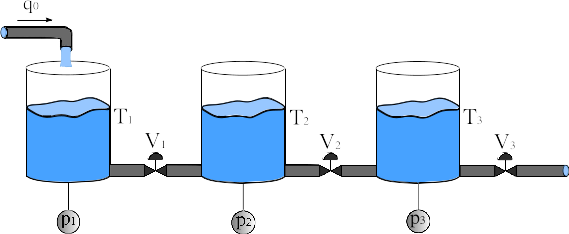
\includegraphics[width=0.5\textwidth]{Tanks.png}
		\end{figure} }


		\itemizespace

		\item[] \alert
		{
			\[
				\frac{\delta {h_1}}{\delta t} = q_0 - q_1 = \frac{q_0-k_1 sign(h_1, h_2) \sqrt{|h_1-h_2|}}{A_1}
			\]

			\[
				\frac{\delta {h_2}}{\delta t} = \frac{k_{1} sign(h_{1}, h_2) \sqrt{|h_{1}-h_2|}-k_2 \sqrt{h_2}}{A_2}
			\]

			\[
				\frac{\delta {h_3}}{\delta t} = \frac{k_{2} sign(h_{2}, h_3) \sqrt{|h_{2}-h_3|}-k_3 \sqrt{h_3}}{A_3} 
			\]

		}

		\itemizespace

		\item[] \alert
		{
			\begin{table}
				\begin{tabular}{ cc }
					Input: $u=\{q_0,v_1,v_2,v_3\}$	&
					Output: $y=\{p_1,p_2,p_3\}$		\\
				\end{tabular}
			\end{table}
		}
	\end{itemize}

\end{frame}

\begin{frame}{Control Model}
	\begin{itemize}
		\item \alert<+>
		{
			Nominal system model:
			\[
				\begin{array}{rcl}
					x_{k+1}	& =	& A_\gamma x_k + B_\gamma u_k + w_k \\
					y_k		& =	& C_\gamma x_k + v_k \\
				\end{array} 
			\]
		}

		\itemizespace

		\item \alert<+>
		{
			Observer model:
			\[
				\begin{array}{rcl}
					\hat{x}_{k+1}	& =	& A_\gamma \hat{x}_k + B_\gamma u_k + L_\gamma (y_k - C_\gamma \hat{x}_k ) \\
					\hat{y}_k		& =	& C_\gamma \hat{x}_k + v_k	\\
					r_k				& = & y_k - C_\gamma \hat{x}_k	\\
					u_k				& = & -K_\gamma \hat{x}_k		\\
				\end{array} 
			\]
		}
	\end{itemize}
\end{frame}

\begin{frame}{External perturbation}
	\begin{itemize}
		\item[]<1->
		{
		\begin{itemize}
				\item \alert<+>
				{
					Faults influence:
					\[
						\begin{array}{rcl}
							x_{k+1}	& =	& A_\gamma x_k + B_\gamma u_k + \textcolor{red}{B_f f_k} + w_k \\
							y_k		& =	& C_\gamma x_k + \textcolor{red}{C_f f_k} + v_k \\
						\end{array} 
					\]
				}

				\itemizespace

				\item \alert<+>
				{
					Attacks influence:
					\[
						\begin{array}{rcl}
							x_{k+1}	& =	& A_\gamma x_k + B_\gamma u_k + \textcolor{red}{B_a a_k} + w_k \\
							y_k		& =	& C_\gamma x_k + \textcolor{red}{D_a a_k} + v_k \\
						\end{array} 
					\]
				}

			\end{itemize}
		}
		\item[]<3-> \alert {\small $f_k$ and $a_k$ are the fault and attack vector respectively.}
	\end{itemize}
\end{frame}

\begin{frame}{Fault Model}

	\begin{itemize}
		\item \alert<+>{Valve faults, leaks, sensor faults, etc..}
		\item \alert<+>{Valve setting: $V_i \in [0,1]$
				\begin{itemize}
					\item $V_i=0$ is closed; $V_i=1$ is open 
					\end{itemize}
		}

		\itemizespace

		\item \alert<+>
		{
			Additive model:
			\[
				v_i =	\begin{cases}
							\max\{0, v_i + \Delta_{v_i}\}, & \mbox{if } \Delta_{v_i} \leq 0 \\
							\min\{1, v_i + \Delta_{v_i}\}, & \mbox{if } \Delta_{v_i} > 0 \\
						\end{cases}
			\]
			where $\Delta_{v_i} \in [-1,1]$

		}

		
    \end{itemize}
\end{frame}

\begin{frame}{Attacks Model}

	\begin{itemize}
		\item \alert<+>{The attacker cannot monitor the system, only data
			injection.}

		\itemizespace

		\item \alert<+>
		{
			\textbf{Sensor:} fake sensor reading in $[0,p_{i}^{max}]$ \\
			%	The system may be altered if the control system responds to the change.
		}

		\itemizespace

		\item \alert<+>
		{
			\textbf{Actuator:} fake actuator position in $[0,1]$ \\
			%	The system is always affected.
		}
    \end{itemize}
\end{frame}

%%%%%%%%%%%%%%%%%%%%%%%%%%%%%%%%%%%%%%%%%%%%%%%%%%%%%%%%%%%%%%%%%%%%%%%%%%%%%%%

\section{Fault or Attack}

\begin{frame}{Fault or Attack}
	\begin{itemize}
		\item \alert<+>
		{
			Our system runs over different modes, each of which has a physical
			model $\psi_i$, creating the behaviour $\xi_i$ having measurement
			$\hat{y_i}$.
		}

		\itemizespace

		\item \alert<+>
		{
			\textbf{Mode estimation:} closest mode to anomalous observation
			$\widetilde{y_i}$
			\[
				\psi^* = arg \min_{\psi_i \in \Psi}{|| \widetilde{y_i} - \hat{y_i} ||} 
						= arg \min_{\psi_i \in \Psi}{r_i} 
			\]
		}

		\itemizespace

		\item \alert<+>
		{
			\textbf{Mode identifiability:} 
			\begin{itemize}
				\item[-] distinguishable behaviour $\xi_i \ \forall j \neq i$
				\item[-] activated residual $r_i > \delta$ if system is in mode
					$\psi_i$
			\end{itemize}
		}

	\end{itemize}
\end{frame}

%%%%%%%%%%%%%%%%%%%%%%%%%%%%%%%%%%%%%%%%%%%%%%%%%%%%%%%%%%%%%%%%%%%%%%%%%%%%%%%

\section{Experimental Results}

\begin{frame}{Experiments}
	\begin{itemize}
		\item \alert<+>
		{
			Three types of tests:
			\begin{itemize}
				\item[-]{Sensors attacks}

				\itemizespace
					
				\item[-]{Actuators attacks}

				\itemizespace
					
				\item[-]{Multiple components attacks}
			\end{itemize}
		}

		\itemizespace

		\item \alert<+>
		{
			Experimental environment:
			\begin{itemize}
				\item[-]{Time domain: $[0,50]$ seconds}

				\itemizespace
					
				\item[-]{Sensor data gathered every 2 seconds}

				\itemizespace
					
				\item[-]{Nominal setting: $v_1=v_2=v_3=0.5$}
			\end{itemize}
		}
	\end{itemize}
\end{frame}

\begin{frame}{Attacks on Sensors}

	\alert{Injected data on the second sensor of our system}

	\begin{columns}
		\begin{column}{0.5\textwidth}
			\begin{figure}
				%	\centering
				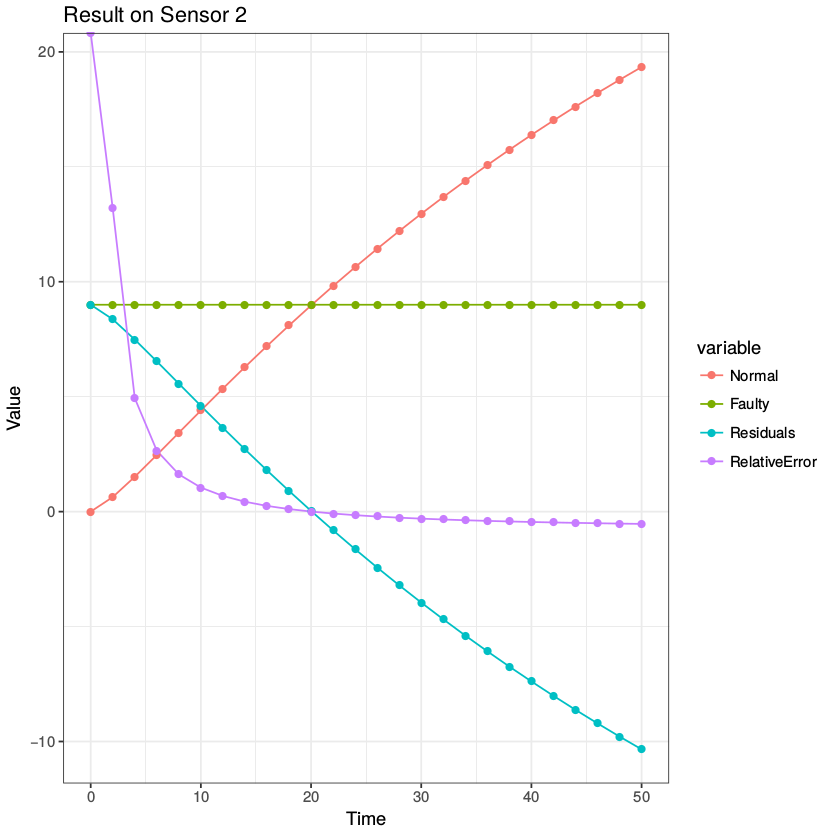
\includegraphics[width=\textwidth]{attack_sensor2_2}
				\label{fig:attack_valve}
			\end{figure}
		\end{column}

		\begin{column}{0.5\textwidth}
			\alert{Attack identified through first derivative comparison:
				\[ \dot{y}_k=-\dot{r}_k \]
			}
		\end{column}
	\end{columns}

\end{frame}

\begin{frame}{Attacks on Actuators}

	\alert{System complexity makes identifiability harder when the actuators are
	under attack, creating false positives.}

	\begin{columns}
		\begin{column}{0.5\textwidth}
			\begin{figure}
				%	\centering
				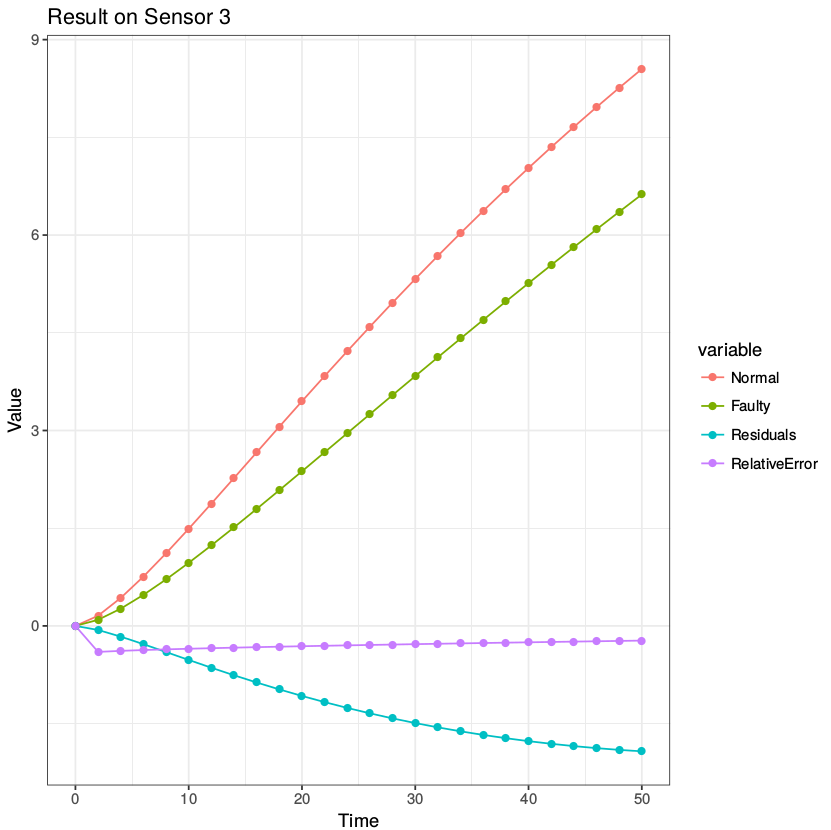
\includegraphics[width=\textwidth]{attack_valve}
				\label{fig:attack_valve}
			\end{figure}
		\end{column}

		\begin{column}{0.5\textwidth}
			\begin{table}
				\alert{
					\tiny
					%	\centering
					\renewcommand{\arraystretch}{1.25}
					\begin{tabular}{ c | ccc }
						Test	&	Valve 1			&	Valve 2		&	Valve 3		\\
						\hline
						155		&	\checkmark		&	X			&	X			\\
						355		&	\checkmark		&	X			&	X			\\
						755		&	\checkmark		&	X			&	X			\\
						955		&	\checkmark		&	X			&	X			\\
						515		&	X				&	\checkmark	&	X			\\
						535		&	X				&	\checkmark	&	X			\\
						575		&	X				&	\checkmark	&	X			\\
						595		&	X				&	\checkmark	&	X			\\
						551		&					&				&	\checkmark	\\
						553		&					&				&	\checkmark	\\
						557		&					&				&	\checkmark	\\
						559		&					&				&	\checkmark	\\
						\hline
						158		&	\checkmark		&	X			&	\checkmark	\\
						544		&	X				&	\checkmark	&	\checkmark	\\
						658		&	\checkmark		&	X			&	\checkmark	\\
						745		&	\checkmark		&	\checkmark	&	X			\\
						958		&	\checkmark		&	X			&	\checkmark	\\
						\hline
						247		&	\checkmark		&	\checkmark	& \checkmark	\\
						638		&	\checkmark		&	\checkmark	& \checkmark	\\
					\end{tabular}
					\label{tab:attack_valve}
				}
			\end{table}
		\end{column}
	\end{columns}

\end{frame}

\begin{frame}{Multi Attacks and Results}
		\alert{Sensors problems correctly detected and identified. \\
		Actuators errors detected. \\  

		\itemizespace

		\tiny
		\begin{table}
			%\centering
			\renewcommand{\arraystretch}{1.25}
			\begin{tabular}{ c | cccc }
				Test		&	Valve 1		&	Valve 2		&	Valve 3		&	Sensor	\\
				\hline
				s1\_325		&				&	\checkmark	&	X			&	1		\\
				s2\_553		&	X			&				&	\checkmark	&	2		\\
				s3\_148		&	\checkmark	&	\checkmark	&				&	3		\\
				\hline
				s12\_558	&				&				&	\checkmark	&	1-2		\\
				s23\_647	&	\checkmark	&				&				&	2-3		\\
				s31\_348	&				&	\checkmark	&				&	1-3		\\
				s123\_666	&				&				&				&	1-2-3	\\
			\end{tabular}
			\label{tab:attack_multi}
		\end{table}
		}

\end{frame}

%%%%%%%%%%%%%%%%%%%%%%%%%%%%%%%%%%%%%%%%%%%%%%%%%%%%%%%%%%%%%%%%%%%%%%%%%%%%%%%

\section{Summary and Conclusions}

\begin{frame}{Summary and Future Work}
    \begin{itemize}
		\item \alert<+>
		{
			Showed a security system approach based on Cyber-Physical Systems.
		}

		\itemizespace

		\item \alert<+>
		{
			Distinguishing attacks from faults is difficult when the system has
			few sensors.
		}

		\itemizespace

		\item \alert<+>
		{
			Future work
			\begin{itemize}
				\item Deeper studies on the synergies of the system and
					between sensors' data.
				\item Optimize the number of sensors in the system.
			\end{itemize}
		}

    \end{itemize}
\end{frame}

\begin{frame}
	\begin{figure}
		
\includegraphics[height=0.6\textheight]{thank-you}
	\end{figure}
\end{frame}

\end{document}

